\documentclass[11pt,a4paper]{ctexart}
\usepackage[teacher]{ipara}
\tcbuselibrary{breakable}
\usepackage{multicol}

\usepackage{pgfplots}
\pgfplotsset{compat=1.18}
\usetikzlibrary{arrows.meta,positioning,decorations.pathreplacing}

\definecolor{mainblue}{RGB}{32,80,145}
\definecolor{lightblue}{RGB}{240,244,249}
\definecolor{maingreen}{RGB}{25,125,90}
\definecolor{lightgreen}{RGB}{240,248,244}
\definecolor{mainorange}{RGB}{218,116,20}
\definecolor{lightorange}{RGB}{254,247,238}
\definecolor{mainred}{RGB}{190,50,55}
\definecolor{lightred}{RGB}{253,241,241}
\definecolor{graybox}{RGB}{247,247,247}

\pagestyle{fancy}
\fancyhf{}
\lhead{\small 高一上：对数函数综合专题知识教案}
\rhead{\small 教师版（结构转化与零点关系）}
\cfoot{\small 第 \thepage\ 页\quad 共 \zpageref{LastPage} 页}
\renewcommand{\headrulewidth}{0.4pt}
\renewcommand{\footrulewidth}{0pt}


\renewcommand{\teacherproblem}[2]{%
  \teachquestionheader{原卷第 #1 题\quad #2}
}

\newcommand{\dd}{\mathrm{d}}
\newcommand{\R}{\mathbb{R}}
\newcommand{\e}{\mathrm{e}}

\begin{document}

\begin{center}
  {\zihao{2}\bfseries 高一上 \quad 对数函数综合专题知识教案}\\[3mm]
  {\Large \bfseries 不用导数的“结构转化”主线}\\[2mm]
  {\large 适用：高一上对数函数综合 / 拔高专题 / 每讲 120 分钟}\\[2mm]
  \rule{0.85\linewidth}{0.5pt}
\end{center}

\begin{teachbox}{课程定位}
本教案是“对数函数综合”专题的知识教案，不是单次错题课教案。
因此内容不按一节 120 分钟压缩，而是按知识阶梯拆成若干个 120 分钟课次连续讲授。

本专题不把这类题统称为“极值点偏移”。严格地说，极值点偏移多属于高三导数专题；高一阶段更合适的板块名称是：
\[
\boxed{\text{对数函数综合：结构转化、图像关系、换元降维与零点关系}}
\]
开课时要先帮学生改名：
\[
\boxed{\text{这些题不是先归入导数的“极值点偏移”，而是高一阶段的结构转化型函数题。}}
\]
本专题的核心不是“算对数”，而是训练学生把文字、图像、对数、指数、二次函数、分式最值和根的关系互相翻译。

可以给学生的第一句话是：
\[
\boxed{\text{对数综合题不是考你会不会算 }\log\text{，而是考你能不能剥掉对数外壳，看见里面真正的函数结构。}}
\]
\end{teachbox}

\begin{teachbox}{学情分析：典型学习断点}
部分学生计算过程认真沉稳、关注细节；但在面对陌生或综合题时，\textbf{对数学模型的构建能力偏弱，对题目条件的几何直观理解不够深刻}，极易机械式套用代数公式，在多步推导的逻辑链条及整体建模思路上存在盲区。
本讲义教案旨在帮助学生：
\begin{enumerate}
  \item \textbf{强化直观翻译}：从几何投影、平行/垂直等直观角度审视解析条件，建立“数形转化”的直觉。
  \item \textbf{规范建模步骤}：将复杂的综合性问题拆解为“画图/找投影 $\to$ 找比值换元 $\to$ 降元求解”等规范的流程模板，并强制补充证明和推理的逻辑中间句。
\end{enumerate}
\end{teachbox}

\section{专题目标、扫描顺序与课时拆分}

\subsection*{一、教学目标}
\begin{enumerate}
  \item 会处理对数函数的“守门条件”：真数大于零、底数合法、单调性方向。
  \item 能把图像语言翻译为函数值关系：在上方、在下方、公共点、恒成立。
  \item 能从坐标变换读出相关函数解析式。
  \item 能用对数运算法则完成“脱壳、合并、换元”。
  \item 能识别“目标反推换元”：出现 $x_1x_2$、$\ln\dfrac{x_1}{x_2}$ 时，优先研究 $\ln x_1,\ln x_2$。
  \item 知道高一方法与高三导数方法的边界：本课不用导数，只讲结构转化、二次函数、基本不等式与单调性。
\end{enumerate}

\subsection*{二、基本功与真正难点}

\begin{teachbox}{教师先统一判断}
这类题的知识点表面并不难：定义域、对数运算、单调性、图像关系、二次函数和基本不等式都属于高一可讲范围。

真正难点不在“会不会背公式”，而在：
\[
\boxed{\text{能不能从题目中看出该构造什么对象、该比较什么量、该换什么元。}}
\]
所以本专题上课时要把学生的能力拆成两层：
\[
\boxed{\text{基本功层：守门、脱壳、单调、图像、放缩}}
\qquad
\boxed{\text{构造层：设元、同构、消参、比较对象、根关系}.}
\]
如果只讲第一层，学生会觉得“都听懂了”；一到综合题仍然不知道第一笔写什么。
\end{teachbox}

\begin{center}
\renewcommand{\arraystretch}{1.25}
\begin{tabularx}{0.95\linewidth}{>{\bfseries}p{2.4cm} X X}
\toprule
层次 & 学生要具备的基本动作 & 本专题真正训练的难点 \\
\midrule
定义域意识 & 带变量先锁定真数、底数、分母、根式范围。 & 把定义域与题目给定区间、换元范围、参数范围合并使用。 \\
单调性意识 & 不用导数时，只用基本函数单调性、复合函数单调性和定义法证明。 & 看出应该构造哪个函数 $F(x)$，再用单调性推出 $F(x_1)=F(x_2)\Rightarrow x_1=x_2$ 或比较大小。 \\
结构运算意识 & 会把对数和差合并，把倍数放进幂，把指数和对数互化。 & 反向识别结构，例如把 $2\ln x+x$ 看成 $\ln(x^2\e^x)$，从而设 $t=x^2\e^x$。 \\
图像翻译意识 & 会把上方、下方、公共点、恒成立翻译成函数值关系。 & 分清主语和区间，把“图像关系”落到不等式、零点个数或参数临界。 \\
根关系意识 & 知道一元二次根与系数关系，知道反函数交点关系。 & 接受“不求根，只求根关系”，用两个零点式消参得到 $x_1x_2$、$x_1+x_2$ 或 $\ln\dfrac{x_1}{x_2}$。 \\
\bottomrule
\end{tabularx}
\end{center}

\begin{keybox}{讲给学生的定位句}
\[
\boxed{\text{这类题不是难在公式，而是难在观察、翻译、构造和组织顺序。}}
\]
高一阶段不借助导数时，我们仍然可以研究函数；但研究方式主要是定义法单调性、基本函数图像、初等凹凸直观、对数放缩、换元降维和零点关系。
\end{keybox}

\subsection*{三、学生拿到题后的“大脑扫描顺序”}

\begin{teachbox}{总扫描句}
对数综合题的稳定入口不是题型名，而是一套动作顺序：
\[
\boxed{
\text{守门}
\to
\text{脱壳合并}
\to
\text{看目标换元}
\to
\text{翻译图像语言}
\to
\text{降成基本函数}
\to
\text{找根与参数关系}.}
\]
课堂上每道题都要求学生先口头说一遍自己走到哪一步，而不是直接写计算。
\end{teachbox}

\begin{center}
\renewcommand{\arraystretch}{1.3}
\begin{tabularx}{0.95\linewidth}{>{\bfseries}p{2.3cm} X X}
\toprule
扫描动作 & 看到什么 & 立刻做什么 \\
\midrule
第0步：守门 & $\log_a M$ & 检查 $a>0,\ a\ne1,\ M>0$；先写定义域。 \\
第1步：脱壳合并 & 同底对数、和差、系数 & 用单调性脱壳；把和差合并为积商；把 $k\log_a x$ 改写为 $\log_a x^k$。 \\
第2步：目标反推换元 & $x_1x_2,\ \ln\dfrac{x_1}{x_2},\ 9^x,3^x$ & 研究 $\ln x_1,\ln x_2$；设 $t=3^x$；把目标式变成变量选择的依据。 \\
第3步：图像语言翻译 & 上方、下方、公共点、任意 $x$、点变换 & 写成 $f(x)>g(x)$、$f(x)=g(x)$ 有解、恒成立、$ly=f(kx)$。 \\
第4步：降成基本函数 & 脱壳后的二次式、分式、均值结构 & 转入二次函数区间问题、分式最值、基本不等式。 \\
第5步：根关系 & 两个根、两个零点、同一个参数 & 不急着求根，先找 $x_1+x_2,\ x_1x_2,\ \ln\dfrac{x_1}{x_2}$ 或参数消去关系。 \\
\bottomrule
\end{tabularx}
\end{center}

\begin{keybox}{给学生的板书口号}
\[
\boxed{\text{先守门，再脱壳；先翻译，再计算；先找结构，再求数。}}
\]
\end{keybox}

\subsection*{四、题型地图}

\begin{center}
\renewcommand{\arraystretch}{1.25}
\begin{tabularx}{0.95\linewidth}{>{\bfseries}p{2.5cm} X X X}
\toprule
题型 & 典型特征 & 核心动作 & 高一可用工具 \\
\midrule
对数脱壳型 & $\log_a A=\log_a B$ 或 $\log_a A<\log_a B$ & 先守门，再脱壳 & 定义域、底数单调性、真数比较 \\
图像变换型 & 点 $M(x,y)$ 变为 $M'(kx,ly)$ & 把坐标对应翻译为解析式 & 坐标代入、相关函数解析式转换 \\
函数比较型 & 图像在上方/下方、恒成立 & 把图像语言翻译为函数值不等式 & 二次函数区间控制、端点临界 \\
指对互逆型 & $a^x=\log_a x$ & 不求根，先看反函数交点 & 反函数、单调性、交点关系 \\
零点关系型 & $f(x_1)=0,\ g(x_2)=0$ & 同一参数先表示两次再消去 & 消参数、结构换元、根关系 \\
指对混合型 & $\e^x,\ln x,x^2$ 同时出现 & 合并、同构、判断是否越界到导数 & 对数合并、同构换元、图像直观 \\
新定义推理型 & 由集合或规则定义函数关系 & 先翻译定义，再做分类与包含证明 & 分段函数、集合包含、反证法 \\
\bottomrule
\end{tabularx}
\end{center}

\subsection*{五、工具分层}

\begin{center}
\renewcommand{\arraystretch}{1.25}
\begin{tabularx}{0.95\linewidth}{>{\bfseries}p{2.4cm} X X}
\toprule
层级 & 必须讲清的工具 & 讲课边界 \\
\midrule
第一层：必讲工具 & 定义域、底数单调性、对数运算、指数对数互化、图像语言翻译、基础换元。 & 每一题都要用，要求学生形成固定检查动作。 \\
第二层：拔高工具 & 反函数交点、零点消参、同构观察、$\ln x$ 基础放缩、对数差估计。 & 可以讲思想和常用结论，但每次必须交代适用条件。 \\
第三层：暂缓工具 & 导数、隐零点、极值点偏移、复杂凸凹性证明、高阶对数平均不等式。 & 可以说明它们与本专题有亲缘关系，但不作为高一正式主线。 \\
\bottomrule
\end{tabularx}
\end{center}

\subsection*{六、四讲课时拆分建议}

\begin{center}
\renewcommand{\arraystretch}{1.25}
\begin{tabularx}{0.95\linewidth}{>{\bfseries}p{2.2cm} p{3.1cm} p{2.1cm} X}
\toprule
课次 & 主题 & 时长 & 内容安排 \\
\midrule
第一讲 & 对数综合的底层规则 & 120 分钟 & 守门条件、底数单调、对数运算、脱壳、合并、基础换元；配合练习1建立“先守门，再脱壳”。 \\
第二讲 & 图像语言与相关函数 & 120 分钟 & 课前热身、坐标变换、相关函数、图像上下关系、恒成立、二次函数端点临界、分式最值；主讲例题1。 \\
第三讲 & 指对互逆与不求根思想 & 120 分钟 & 指数对数互为反函数、递增函数与反函数交点、根关系不变量；主讲例题2，训练“不求根也能求根关系”。 \\
第四讲 & 零点消参与结构换元 & 120 分钟 & 零点消参、结构块换元、$q$ 比值降维、$\ln x$ 放缩、同构观察；主讲例题3，例题4作为逻辑推理拓展。 \\
\bottomrule
\end{tabularx}
\end{center}

\subsection*{七、四讲基础原理与问题链}

\begin{teachbox}{第一讲：对数综合的底层规则}
\textbf{要讲清的基础原理：}
\[
\log_a M \text{ 有意义}\Longleftrightarrow a>0,\ a\ne1,\ M>0.
\]
\[
a>1:\log_a x \text{ 递增};\qquad 0<a<1:\log_a x \text{ 递减}.
\]
\[
\log_a MN=\log_a M+\log_a N,\qquad
\log_a\frac MN=\log_a M-\log_a N,\qquad
k\log_a M=\log_a M^k.
\]
第一讲不追求难度，追求动作稳定。
学生必须知道：脱壳前先守门，脱壳时看底数，换元后写范围。

\textbf{问题链：}
\begin{enumerate}
  \item 这道题所有对数的真数是什么？底数是否合法？
  \item 底数大于 $1$ 还是小于 $1$？不等号方向变不变？
  \item 对数能不能合并？能不能脱壳？
  \item 换元后新变量的范围是什么？
\end{enumerate}
\end{teachbox}

\begin{teachbox}{第二讲：图像语言与相关函数}
\textbf{要讲清的基础原理：}
\[
\text{图像 } y=f(x)\text{ 在 }y=g(x)\text{ 下方}
\Longleftrightarrow
f(x)<g(x).
\]
\[
\text{仅有一个公共点}
\Longleftrightarrow
f(x)=g(x)\text{ 只有一个根}.
\]
若 $M(x,y)$ 在 $y=g(x)$ 上，且 $M'(kx,ly)$ 在 $y=f(x)$ 上，则
\[
y=g(x),\qquad ly=f(kx),\qquad
\boxed{g(x)=\frac1l f(kx).}
\]
相关函数题的难点不是公式，而是坐标对应方向。
例题1脱壳后会落到二次函数恒成立和分式最值，这正是“对数外壳，函数内核”的典型。

\textbf{问题链：}
\begin{enumerate}
  \item “图像在下方”的主语是谁？
  \item $M'(3x,2y)$ 在 $y=f(x)$ 上，应写 $2y=f(3x)$ 还是 $g(3x)=2f(x)$？
  \item “任意 $x\in(0,1)$”转成什么恒成立问题？
  \item 开区间端点为什么可以允许等号？
  \item 绝对值打开后，最大值问题落到了哪个基本函数？
\end{enumerate}
\end{teachbox}

\begin{teachbox}{第三讲：指对互逆与不求根思想}
\textbf{要讲清的基础原理：}
当 $a>0,\ a\ne1$ 时，
\[
y=a^x\quad \Longleftrightarrow \quad x=\log_a y.
\]
所以 $y=a^x$ 与 $y=\log_a x$ 的图像关于 $y=x$ 对称。
若 $\varphi(x)$ 严格递增且存在反函数，则
\[
\varphi(x)=\varphi^{-1}(x)
\quad \Longrightarrow \quad
\varphi(x)=x.
\]
因此对于 $c>1$，
\[
c^x=\log_c x
\quad \Longrightarrow \quad
c^x=x.
\]
例题2的核心不是求出 $a,b$，而是把两个根转化为
\[
c^a=a,\qquad c^b=b,\qquad ab=c^{a+b}.
\]

\textbf{问题链：}
\begin{enumerate}
  \item 指数函数和对数函数互为反函数，图像上意味着什么？
  \item 为什么这里必须强调 $c>1$？
  \item 题目要求根的具体值，还是根之间的不变量？
  \item 不求 $a,b$，我们能得到 $ab$ 和 $a+b$ 的什么关系？
\end{enumerate}
\end{teachbox}

\begin{teachbox}{第四讲：零点消参、结构换元与同构}
\textbf{要讲清的基础原理：}
看到
\[
f(x_1)=0,\qquad g(x_2)=0
\]
且两个方程含同一个参数 $t$，先做：
\[
\boxed{
\text{由第一个零点表示 }t
\to
\text{由第二个零点表示 }t
\to
\text{令两式相等}.}
\]
这叫零点消参。
例题3中天然出现
\[
1+\ln x_1,\qquad -\ln x_2,
\]
所以设
\[
u=1+\ln x_1,\qquad v=-\ln x_2,\qquad q=\frac uv.
\]
换元不是拍脑袋，而是被目标式和重复结构逼出来的。

\textbf{$\ln x$ 放缩要按场景选择：}
\[
\ln x\le x-1,\qquad
\ln x\ge \frac{x-1}{x},
\]
\[
\ln(1+t)\le t,\qquad
\ln(1+t)\ge \frac{t}{1+t}\quad(t\ge0),
\]
\[
0<a<b:\qquad
\frac{b-a}{b}<\ln\frac ba<\frac{b-a}{a}.
\]
如果出现两个变量的对数差，再考虑对数平均：
\[
\sqrt{x_1x_2}
<
\frac{x_1-x_2}{\ln x_1-\ln x_2}
<
\frac{x_1+x_2}{2}.
\]

\textbf{同构要讲四种入口：}
\begin{enumerate}
  \item 不同变量在两侧：整理成 $F(x_1)=F(x_2)$。
  \item 题目给出等式：设 $t=A(x)=B(y)$。
  \item 含参与不含参分离：由零点式整理成 $a=\Psi(x)$。
  \item 指数对数互化：用 $x=\ln \e^x,\ k\ln x=\ln x^k,\ y=a^x\Longleftrightarrow x=\log_a y$。
\end{enumerate}

\textbf{问题链：}
\begin{enumerate}
  \item 两个零点方程里共同参数是谁？
  \item 能不能分别把这个参数表示出来？
  \item 方程中反复出现的结构块是什么？
  \item 目标是 $x_1x_2$ 还是 $\ln\dfrac{x_1}{x_2}$？它提示我们研究什么？
  \item 写成 $\Phi(A)=\Phi(B)$ 后，还差哪一句严谨性说明？
\end{enumerate}
\end{teachbox}

\begin{keybox}{一句话主线}
\[
\boxed{\text{对数外壳}\to\text{结构翻译}\to\text{基本函数}\to\text{根与参数关系}.}
\]
\end{keybox}

\section{课前必须统一的“观察清单”}

\begin{multicols}{2}
\begin{keybox}{观察1：守门条件}
\[
\log_a M \text{ 有意义}\Longleftrightarrow a>0,\ a\ne1,\ M>0.
\]
尤其在含参题中，真数条件常常给出参数范围。
\end{keybox}

\begin{keybox}{观察2：单调性方向}
\[
 a>1: \log_a x \text{递增};\qquad 0<a<1: \log_a x \text{递减}.
\]
比较对数大小前，先看底数。
\end{keybox}

\begin{keybox}{观察3：对数合并}
\[
\log_a M+\log_a N=\log_a(MN),
\]
\[
\log_a M-\log_a N=\log_a\frac{M}{N},
\qquad k\log_a M=\log_a M^k.
\]
\end{keybox}

\begin{keybox}{观察4：目标反推换元}
若目标出现
\[
x_1x_2,\quad \frac{x_1}{x_2},\quad \ln\frac{x_1}{x_2},
\]
优先想到
\[
\ln(x_1x_2)=\ln x_1+\ln x_2,
\qquad
\ln\frac{x_1}{x_2}=\ln x_1-\ln x_2.
\]
\end{keybox}
\end{multicols}

\begin{warnbox}{高一阶段不要滥用的词}
这些题和高三“隐零点、极值点偏移”有亲缘关系，但不能全部叫极值点偏移。高一阶段推荐称作：
\[
\boxed{\text{对数结构转化型函数综合题}}
\]
因为本课不求导，主要靠对数运算、单调性、二次函数、换元和图像语言翻译。
\end{warnbox}

\section{课前热身：从投影直觉到几何建模}

\begin{teachbox}{设计意图}
利用该几何与解三角形热身题，引导学生跳出机械套用“余弦定理”的代数计算思维，体验通过“作高投影”获得更直观几何路径的过程。同时在第(2)问中，练习在平行与垂直的复杂线条中，寻找角的互补与互余关系，逐步引导学生建立“化未知为已知”的平面解三角形建模路径。
\end{teachbox}

\subsection{热身题：解三角形与投影法}

\begin{exbox}{热身题}
已知在 $\triangle ABC$ 中，$AB=3$，$BC=2\sqrt3$，$\cos B=\dfrac{\sqrt3}{3}$。
\begin{enumerate}[label=(\arabic*)]
  \item 求 $\cos A$；
  \item 设 $D, E$ 两点满足：$D$ 在 $BA$ 的延长线上，$DE\parallel BC$，$AE\perp AC$。若 $DE=\sqrt6$，求 $CE$。
\end{enumerate}
\end{exbox}

\begin{center}
\begin{tikzpicture}[scale=1.0, >=stealth, line join=round, line cap=round]
  % 顶点坐标
  \coordinate (A) at (0,0);
  \coordinate (B) at (3,0);
  \coordinate (C) at (1, 2.828);
  \coordinate (D) at (-4.242, 0);
  \coordinate (E) at (-5.657, 2);
  
  % 绘制三角形与延长线
  \draw[thick] (D) -- (B) -- (C) -- (A);
  \draw[thick] (D) -- (E);
  \draw[thick, mainblue] (A) -- (E);
  \draw[thick, mainred] (C) -- (E);
  
  % 标注直角 (AE \perp AC)
  \coordinate (AE_dir) at (-0.943, 0.333); % unit vector along AE
  \coordinate (AC_dir) at (0.333, 0.943); % unit vector along AC
  \draw[gray] ($(A) + 0.3*(AE_dir)$) -- ($(A) + 0.3*(AE_dir) + 0.3*(AC_dir)$) -- ($(A) + 0.3*(AC_dir)$);

  % 教师端增加辅助线 (垂足 H)
  \ifteacher
    \coordinate (H) at (1,0);
    \draw[dashed, gray!80, thick] (C) -- (H);
    \node[below] at (H) {\small $H$};
    \draw[gray] (0.8,0) -- (0.8,0.2) -- (1,0.2);
  \fi

  % 顶点字母
  \node[below] at (A) {$A$};
  \node[below right] at (B) {$B$};
  \node[above] at (C) {$C$};
  \node[below left] at (D) {$D$};
  \node[above left] at (E) {$E$};
\end{tikzpicture}
\end{center}

\begin{paracol}{2}
\teachblock{标准解答与讲解主线}{
  \textbf{第(1)问：高线投影法（推荐主讲）}\\
  已知 $\cos B = \dfrac{\sqrt{3}}{3}$，这表示边 $BC$ 在 $BA$ 方向上的投影。\\
  作 $CH \perp AB$ 于 $H$。\\
  在 Rt$\triangle BCH$ 中：
  \[
  BH = BC \cos B = 2\sqrt{3} \cdot \frac{\sqrt{3}}{3} = 2.
  \]
  因为 $AB = 3$，所以 $AH = AB - BH = 3 - 2 = 1$。\\
  又由勾股定理：
  \[
  CH^2 = BC^2 - BH^2 = 12 - 4 = 8 \implies CH = 2\sqrt{2}.
  \]
  In Rt$\triangle ACH$ 中：
  \[
  AC = \sqrt{AH^2 + CH^2} = \sqrt{1^2 + 8} = 3.
  \]
  从而：
  \[
  \cos A = \frac{AH}{AC} = \boxed{\frac{1}{3}}.
  \]
  
  \textbf{余弦定理对比（备选解法）}\\
  在 $\triangle ABC$ 中，由余弦定理：
  \[
  AC^2 = AB^2 + BC^2 - 2AB \cdot BC \cos B = 9 + 12 - 2 \cdot 3 \cdot 2\sqrt{3} \cdot \frac{\sqrt{3}}{3} = 9.
  \]
  解得 $AC = 3$。再次使用余弦定理：
  \[
  \cos A = \frac{AB^2 + AC^2 - BC^2}{2AB \cdot AC} = \frac{9 + 9 - 12}{2 \cdot 3 \cdot 3} = \frac{6}{18} = \frac{1}{3}.
  \]
  \textbf{讲解建议}：引导学生发现，做投影只需简单的一步勾股定理和投影长度计算，省去了余弦定理中繁琐的乘法与根式运算。这表明：\textbf{读懂条件的几何意义（如 $\cos B$ 表示投影）往往能提供更优的路线}。

  \textbf{第(2)问：解三角形几何建模}\\
  第一步：观察角的关系，将已知角平移至目标三角形 $\triangle ADE$。\\
  因为 $DE \parallel BC$，且 $D, A, B$ 三点共线，所以 $\angle ADE$ 与 $\angle B$ 互补，即：
  \[
  \angle ADE = 180^\circ - B \implies \sin\angle ADE = \sin B.
  \]
  由(1)知 $\cos B = \dfrac{\sqrt{3}}{3}$，则 $\sin B = \sqrt{1-\cos^2 B} = \dfrac{\sqrt{6}}{3}$。\\
  又因为 $AE \perp AC$，且 $D, A, B$ 三点共线，所以 $\angle DAE$ 与 $\angle A$ 互余，即：
  \[
  \angle DAE = 90^\circ - A \implies \sin\angle DAE = \cos A = \frac{1}{3}.
  \]
  第二步：在 $\triangle ADE$ 中利用正弦定理求 $AE$。\\
  由正弦定理 $\dfrac{AE}{\sin\angle ADE} = \dfrac{DE}{\sin\angle DAE}$ 得：
  \[
  AE = DE \cdot \frac{\sin\angle ADE}{\sin\angle DAE} = \sqrt{6} \cdot \frac{\frac{\sqrt{6}}{3}}{\frac{1}{3}} = 6.
  \]
  第三步：在 Rt$\triangle ACE$ 中勾股求 $CE$。\\
  因为 $AE \perp AC$，所以 $\triangle ACE$ 是以 $A$ 为直角的直角三角形。\\
  由勾股定理：
  \[
  CE = \sqrt{AC^2 + AE^2} = \sqrt{3^2 + 6^2} = \sqrt{45} = \boxed{3\sqrt{5}}.
  \]
}

\switchcolumn
\teachblock{课堂启发与追问}{
  1. \textbf{直觉引导}：
     “在 $\triangle ABC$ 中，直接给出 $\cos B = \dfrac{\sqrt{3}}{3}$，在直角三角形中它代表什么？我们能不能不通过长公式，直接用画图投影画出它？”
  2. \textbf{建模突破}：
     “我们最终要算 $CE$，它在哪一个三角形中？这个三角形目前已知什么条件？（已知 $AC=3, AE \perp AC$）还缺什么？（缺 $AE$）那 $AE$ 又是哪一个三角形的边？（$\triangle ADE$）在这个三角形中，我们能找出几个角的关系？”
  3. \textbf{追问论证}：
     “为什么 $\angle ADE = 180^\circ - B$？我们在纸上写步骤时，必须先声明哪一条平行关系？”
}
\end{paracol}

\newpage

\section{第一模块：图像语言如何翻译成代数语言}

\begin{teachbox}{教师导入提问}
“图像在下方”是什么？“仅有一个公共点”是什么？“点 $M(x,y)$ 变成 $M'(3x,2y)$”又是什么？很多学生卡住不是因为算力不够，而是因为没有把中文翻译成数学。
\end{teachbox}

\subsection{定理1：坐标变换生成相关函数}

\begin{keybox}{相关函数翻译公式}
若点 $M(x,y)$ 在 $y=g(x)$ 上，且对应点 $M'(kx,ly)$ 在 $y=f(x)$ 上，则
\[
y=g(x),\qquad ly=f(kx),
\]
所以
\[
\boxed{g(x)=\frac1l f(kx)}.
\]
\end{keybox}

\begin{center}
\begin{tikzpicture}[scale=0.9,>=Stealth]
  \draw[->] (-0.5,0)--(6,0) node[right]{$x$};
  \draw[->] (0,-0.5)--(0,4) node[above]{$y$};
  \draw[mainblue, thick, domain=0.2:4.8, smooth, variable=\x] plot ({\x},{1+0.55*ln(\x+0.5)});
  \node[mainblue] at (4.7,3.0) {$y=g(x)$};
  \fill[maingreen] (1.5,1.7) circle (2pt) node[above left]{$M(x,y)$};
  \draw[->, thick, mainorange] (1.7,1.8).. controls (2.7,3.0)..(4.5,3.4);
  \fill[mainorange] (4.5,3.4) circle (2pt) node[above right]{$M'(3x,2y)$};
  \node at (3.1,0.55) {坐标被放大：横坐标 $\times3$，纵坐标 $\times2$};
\end{tikzpicture}
\end{center}

\subsection{例题1：相关函数、图像上下关系与最值}

\begin{exbox}{例题1}
已知函数
\[
f(x)=\log_2(x+a)\quad (a>0).
\]
当点 $M(x,y)$ 在函数 $y=g(x)$ 的图像上运动时，对应点 $M'(3x,2y)$ 在函数 $y=f(x)$ 的图像上运动，称 $y=g(x)$ 是 $y=f(x)$ 的相关函数。
\begin{enumerate}[label=(\arabic*)]
  \item 解不等式 $f(x)<1$；
  \item 对任意 $x\in(0,1)$，$f(x)$ 的图像总在其相关函数图像的下方，求 $a$ 的取值范围；
  \item 设 $F(x)=f(x)-g(x)$，$x\in(0,1)$，当 $a=1$ 时，求 $|F(x)|$ 的最大值。
\end{enumerate}
\end{exbox}

\begin{paracol}{2}
\teachblock{解题路线与标准解答}{
  \textbf{相关函数解析式}：\\
  由坐标变换公式，点 $M(x,y)$ 在 $y=g(x)$ 的图像上，对应点 $M'(3x,2y)$ 在 $y=f(x)$ 的图像上。\\
  由 $2y=f(3x) \implies 2g(x)=f(3x)$，代入得：
  \[
  \boxed{g(x)=\frac12\log_2(3x+a)}.
  \]

  \textbf{第(1)问：守门条件加单调性}：\\
  即为 $\log_2(x+a)<1$。由于底数 $2>1$，且真数要大于零，故：
  \[
  0<x+a<2 \implies \boxed{-a<x<2-a}.
  \]
  \begin{center}
  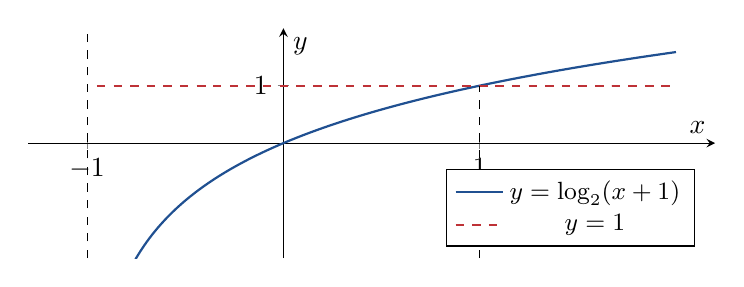
\begin{tikzpicture}
  \begin{axis}[
    width=0.85\linewidth,height=4.5cm,
    axis lines=middle,
    xmin=-1.3,xmax=2.2,ymin=-2,ymax=2,
    xlabel={$x$},ylabel={$y$},
    xtick={-1,0,1},ytick={1},
    samples=200,domain=-0.95:2,
    legend style={at={(0.97,0.05)},anchor=south east,font=\small}
  ]
  \addplot[mainblue,thick] {ln(x+1)/ln(2)};
  \addlegendentry{$y=\log_2(x+1)$}
  \addplot[dashed,mainred,thick] {1};
  \addlegendentry{$y=1$}
  \draw[dashed] (axis cs:-1,-2)--(axis cs:-1,2);
  \draw[dashed] (axis cs:1,-2)--(axis cs:1,1);
  \end{axis}
  \end{tikzpicture}
  \end{center}

  \textbf{第(2)问：图像在下方 $\Rightarrow$ 函数值小}：\\
  题意翻译为对任意 $x\in(0,1)$，有 $f(x)<g(x)$。代入得：
  \[
  \log_2(x+a)<\frac12\log_2(3x+a) \implies \log_2(x+a)^2<\log_2(3x+a).
  \]
  底数 $2>1$ 递增，脱去对数：
  \[
  (x+a)^2<3x+a \implies x^2+(2a-3)x+a^2-a<0.
  \]
  设 $h(x)=x^2+(2a-3)x+a^2-a$。若要在开区间 $(0,1)$ 内恒小于 $0$，只需控制端点：
  \[
  \begin{cases}
    h(0)\le0 \implies a^2-a\le0 \implies 0<a\le1 \\
    h(1)\le0 \implies a^2+a-2\le0 \implies 0<a\le1
  \end{cases}
  \]
  综上所述，得 $\boxed{0<a\le1}$。
  \begin{center}
  \begin{tikzpicture}
  \begin{axis}[
    width=0.8\linewidth,height=4.2cm,
    axis lines=middle,
    xmin=-0.35,xmax=1.35,ymin=-0.35,ymax=0.35,
    xlabel={$x$},ylabel={$h(x)$},
    xtick={0,1},ytick={0},
    samples=120,domain=-0.2:1.2
  ]
  \addplot[mainorange,thick] {x*(x-1)};
  \addplot[mainblue,very thick,domain=0:1] {x*(x-1)};
  \draw[dashed] (axis cs:0,-0.35)--(axis cs:0,0.05);
  \draw[dashed] (axis cs:1,-0.35)--(axis cs:1,0.05);
  \node at (axis cs:0.5,-0.22) {\small $(0,1)$ 内在 $x$ 轴下方};
  \end{axis}
  \end{tikzpicture}
  \end{center}

  \textbf{第(3)问：绝对值打开，再转化为分式最值}：\\
  当 $a=1$ 时，由(2)知在 $x\in(0,1)$ 上有 $f(x)<g(x)$。故：
  \[
  |F(x)|=g(x)-f(x)=\frac12\log_2(3x+1)-\log_2(x+1) = \frac12\log_2\frac{3x+1}{(x+1)^2}.
  \]
  只需求 $R(x)=\frac{3x+1}{(x+1)^2}$ 在 $(0,1)$ 上的最大值。\\
  设 $t=x+1 \in (1,2)$，则：
  \[
  R(x)=\frac{3t-2}{t^2}=\frac3t-\frac2{t^2}.
  \]
  再设 $u=\frac1t \in \left(\frac12,1\right)$，得：
  \[
  R=3u-2u^2=-2\left(u-\frac34\right)^2+\frac98.
  \]
  当 $u=\frac34 \in \left(\frac12,1\right)$ 时，有 $R_{\max}=\frac98$。\\
  此时 $|F(x)|_{\max}=\frac12\log_2\frac98=\log_2\frac{3\sqrt2}{4}$。
}

\switchcolumn
\teachblock{学情诊断与易错点}{
  \begin{itemize}
    \item \textbf{变换关系反向}：容易由 $M'(3x,2y)$ 误推出 $g(3x)=2f(x)$，没有深刻理解坐标代入的对应方向。
    \item \textbf{遗漏定义域（守门条件）}：第(1)问解对数不等式脱壳时，极易只写 $x+a<2$，忽略了真数大于零的条件（$x+a>0$）。
    \item \textbf{区间端点盲目取严格}：在第(2)问控制开口向上的二次函数在开区间 $(0,1)$ 内恒为负值时，经常错写为 $h(0)<0, h(1)<0$。必须强调：端点在开区间外，故端点值取 $0$ 时区间内仍然严格小于 $0$。
    \item \textbf{换元遗漏范围限制}：第(3)问将 $x+1$ 换元为 $t$ 后，极易漏写新变量 $t \in (1,2)$，导致二次函数在区间外的最大值算错。
  \end{itemize}
}

\teachblock{课堂处理与落实建议}{
  1. \textbf{端点临界图示}：在课堂上利用图示说明开区间端点可取等号的物理意义（即使端点在 $x$ 轴上，开区间内部依然完全在 $x$ 轴下方）。
  2. \textbf{强化“脱壳三步骤”}：比较对数前必须：(1) 确定定义域；(2) 比对底数与单调性；(3) 脱壳求解。
}
\end{paracol}

\section{第二模块：反函数交点型，不求根也能求关系}

\begin{teachbox}{教师导入}
有些题看似要求两个根 $a,b$，但根本不需要求根。关键是从“函数与反函数的交点”里拿到根的关系。
\end{teachbox}

\subsection{定理2：增函数与反函数的交点}

\begin{keybox}{反函数交点定理}
若 $y=\varphi(x)$ 是严格增函数，且有反函数 $y=\varphi^{-1}(x)$，则方程
\[
\varphi(x)=\varphi^{-1}(x)
\]
的解一定满足
\[
\boxed{\varphi(x)=x}.
\]
也就是说，增函数与其反函数的交点都在直线 $y=x$ 上。
\end{keybox}

\begin{graynote}
证明思路：设 $y=\varphi(x)=\varphi^{-1}(x)$，则 $\varphi(y)=x$。若 $y>x$，由 $\varphi$ 递增得 $\varphi(y)>\varphi(x)=y$，即 $x>y$，矛盾。若 $y<x$ 同理矛盾。所以 $y=x$。
\end{graynote}

\subsection{例题2：指数与对数互逆}

\begin{exbox}{例题2}
已知两个不相等的正实数 $a,b$ 均满足方程
\[
\left(\frac43\right)^x=\log_{\frac43}x,
\]
求
\[
(a+b)\log_{ab}\frac34.
\]
\end{exbox}

\begin{paracol}{2}
\teachblock{标准解答}{
  设底数 $c=\frac{4}{3}$。\\
  显然，方程 $\left(\frac{4}{3}\right)^x=\log_{\frac{4}{3}}x$ 的解即为函数 $y=c^x$ 与其反函数 $y=\log_c x$ 图像的交点横坐标。\\
  因为底数 $c = \frac{4}{3} > 1$，所以 $y=c^x$ 在其定义域上为严格单调递增函数。\\
  根据反函数交点定理，严格单调增函数与其反函数的交点必然落在直线 $y=x$ 上。\\
  因此，方程的两个不相等正实数根 $a,b$ 必然满足：
  \[
  c^a = a, \qquad c^b = b.
  \]
  两式相乘得：
  \[
  ab = c^a \cdot c^b = c^{a+b}.
  \]
  因此，目标式可变形为：
  \[
  \log_{ab}\frac{3}{4} = \log_{c^{a+b}}c^{-1} = -\frac{1}{a+b}\log_c c = -\frac{1}{a+b}.
  \]
  故所求值为：
  \[
  \boxed{(a+b)\log_{ab}\frac{3}{4} = -1}.
  \]
  \begin{center}
  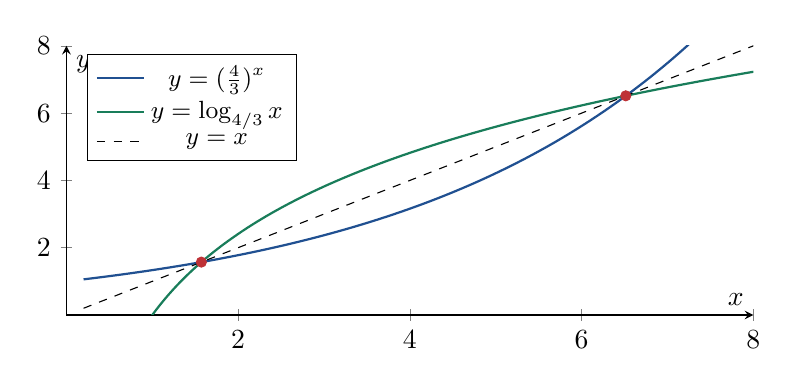
\begin{tikzpicture}
  \begin{axis}[
    width=0.85\linewidth,height=5cm,
    axis lines=middle,
    xmin=0,xmax=8,ymin=0,ymax=8,
    xlabel={$x$},ylabel={$y$},
    xtick={0,2,4,6,8},ytick={0,2,4,6,8},
    samples=260,domain=0.2:8,
    legend style={at={(0.03,0.97)},anchor=north west,font=\small}
  ]
  \addplot[mainblue,thick] {(4/3)^x};
  \addlegendentry{$y=(\frac43)^x$}
  \addplot[maingreen,thick] {ln(x)/ln(4/3)};
  \addlegendentry{$y=\log_{4/3}x$}
  \addplot[dashed,black] {x};
  \addlegendentry{$y=x$}
  \addplot[only marks,mark=*,mark size=1.8pt,mainred] coordinates {(1.5717,1.5717) (6.5139,6.5139)};
  \end{axis}
  \end{tikzpicture}
  \end{center}
}

\switchcolumn
\teachblock{学情诊断与教学要点}{
  \begin{itemize}
    \item \textbf{盲目求根}：许多高一学生看到方程后尝试解出 $a$ 和 $b$ 的具体数值，导致在非初等方程前受挫，无法建立“交点几何位置”与“根的代数方程”之间的转化通道。
    \item \textbf{定理适用边界模糊}：学生容易死记“指对交点必在 $y=x$ 上”，需强调这仅对底数 $c>1$（严格递增）成立；若底数 $0<c<1$（递减），则交点不一定在 $y=x$ 上（可能关于 $y=x$ 对称成对出现）。
  \end{itemize}
}

\teachblock{课堂处理与启发追问}{
  1. \textbf{主线引导}：引导学生通过“反函数”这一触发词进行结构观察，建立“底数相同且指对混合 $\to$ 寻找反函数关系 $\to$ 交点落在 $y=x$ 上”的建模逻辑。
  2. \textbf{启发追问}：
     \begin{itemize}
       \item “如果把底数 $\frac{4}{3}$ 换成 $\frac{1}{2}$，它的交点还一定在 $y=x$ 上吗？为什么？”（引导高分学生思考单调性对反函数交点的影响）
       \item “我们在求解过程中，到底有没有求出 $a$ 和 $b$ 的具体数值？为什么不求也能得出乘积与和的关系？”
     \end{itemize}
}
\end{paracol}

\section{第三模块：零点关系型，先消参数再换元}

\subsection{核心方法：不用导数处理双变量问题的四大套路}

\teachblock{引言}{
面对 $x_1, x_2$ 这种双变量问题，如果不依赖高三的“求导构造单调性”，我们主要依靠\textbf{“代数降维”}和\textbf{“不等式放缩”}。这恰恰是高中数学中最核心的代数变形思维，也是适合高一、高二学生的“正路”。
下面总结不用导数处理双变量问题的四大核心套路：
}

\teachblock{一、 比值换元法（单变量化）}{
这是双变量问题最基础、也最常用的无导数降维方法。当式子具有“齐次”特征，或者可以硬凑出同构的比例时，通过设比值来消灭一个变量。
\begin{itemize}
  \item \textbf{核心动作}：看到式子里多次出现 $x_1, x_2$，直接令 $t = \frac{x_1}{x_2}$（假设 $x_1 > x_2 > 0$，则 $t > 1$）。
  \item \textbf{适用场景}：类似于 $x_1 \ln x_2 - x_2 \ln x_1 = 0$ 或者求 $\frac{x_1 - x_2}{x_1 + x_2}$ 的范围。
  \item \textbf{效果}：两边同除以 $x_2$（或其相关项），原本复杂的双变量问题瞬间化为关于单变量 $t$ 的函数，进而通过二次函数、对数函数的单调性直接解决。
\end{itemize}
}

\teachblock{二、 对数平均不等式（指对双变量的“外挂”）}{
这是处理涉及对数的双变量不等式时，最有效的非导数工具。很多需要构造差值函数求导的题目，用它只需数行即可完成证明。
\begin{itemize}
  \item \textbf{核心公式}：对于任意 $x_1 \neq x_2$ 且 $x_1, x_2 > 0$，必定成立：
  \[
  \sqrt{x_1 x_2} < \frac{x_1 - x_2}{\ln x_1 - \ln x_2} < \frac{x_1 + x_2}{2}
  \]
  \item \textbf{适用场景}：题目已知 $f(x_1) = f(x_2)$（常可推导出 $\ln x_1 - \ln x_2$ 的结构），要求证明 $x_1 + x_2 > 2$ 或 $x_1 x_2 < 1$ 等。
  \item \textbf{本质}：它将“对数差（$\ln x_1 - \ln x_2$）”与“算术平均数（$\frac{x_1+x_2}{2}$）”、“几何平均数（$\sqrt{x_1 x_2}$）”直接建立起代数桥梁，省去了构造差值函数并求导放缩的步骤。
\end{itemize}
}

\teachblock{$\ln x$ 常见放缩工具箱}{
这部分建议在例题3前作为教师板书补充。
核心不是让学生一次背完，而是让学生知道每条放缩解决哪一种问题。

\begin{center}
\renewcommand{\arraystretch}{1.35}
\begin{tabularx}{0.95\linewidth}{>{\bfseries}p{3.4cm} X X}
\toprule
放缩形式 & 使用场景 & 课堂提示 \\
\midrule
$\ln x\le x-1$ & 需要把 $\ln x$ 放大为一次式，常用于证明上界。 & “对数在 $x=1$ 处的切线下方。” \\
$\ln x\ge \dfrac{x-1}{x}$ & 需要给 $\ln x$ 找下界，或式中有 $\dfrac1x$。 & “把 $\ln x$ 与倒数结构接起来。” \\
$\ln(1+t)\le t$ & 出现 $1+t$，且要把对数拆成线性量。 & “靠近 $1$ 的最常用上界。” \\
$\ln(1+t)\ge \dfrac{t}{1+t}$，$t\ge0$ & 出现 $1+t$，且需要下界。 & “分母 $1+t$ 不能漏。” \\
$\dfrac{b-a}{b}<\ln\dfrac ba<\dfrac{b-a}{a}$ & 比较两个正数的对数差。 & “对数差等于割线面积，端点斜率夹住它。” \\
$\sqrt{xy}<\dfrac{x-y}{\ln x-\ln y}<\dfrac{x+y}{2}$ & 双变量题中把对数差转化为平均数关系。 & “这是对数平均，不是普通均值。” \\
\bottomrule
\end{tabularx}
\end{center}

\textbf{板书顺序建议：}
先讲 $\ln x\le x-1$ 和 $\ln(1+t)\le t$，这是学生最常用也最容易接受的上界。
再讲 $\ln x\ge\dfrac{x-1}{x}$，用于需要下界的题。
最后再讲对数差和对数平均，放在 $x_1,x_2$ 双变量问题中使用。

\textbf{易错提醒：}
\begin{itemize}
  \item $\ln x\le x-1$ 是所有 $x>0$ 成立，不需要 $x>1$。
  \item $\ln(1+t)\le t$ 的条件是 $t>-1$，因为真数要大于零。
  \item $\ln(1+t)\ge\dfrac{t}{1+t}$ 常用时取 $t\ge0$，不要在没有检查范围时乱用。
  \item 对数差型必须先统一大小，例如设 $0<a<b$，否则不等号方向容易写反。
\end{itemize}
}

\teachblock{三、 均值不等式及配凑放缩（回归代数本源）}{
不要迷信导数，高中数学的不等式基础是均值不等式及其变形。
\begin{itemize}
  \item \textbf{核心工具}：$a+b \ge 2\sqrt{ab}$，$a^2+b^2 \ge 2ab$ 及其变形。
  \item \textbf{适用场景}：当双变量之间通过方程（如 $x_1 + \ln x_1 = x_2 + \ln x_2$ 等变形式）产生了某种对称关系时。
  \item \textbf{高阶变形}：若 $x_1, x_2$ 是某二次方程的两个根，通过韦达定理得到 $x_1+x_2 = m$，$x_1 x_2 = n$。然后将目标式转化为关于 $m$ 和 $n$ 的关系，变成纯粹的代数计算。
\end{itemize}
}

\teachblock{四、 几何意义法（斜率与凸凹性）}{
有些双变量问题，实质是具有几何背景的斜率问题。
\begin{itemize}
  \item \textbf{核心动作}：看到 $\frac{f(x_1) - f(x_2)}{x_1 - x_2}$，立刻联想到这是图象上两点割线的斜率。
  \item \textbf{适用场景}：题目中出现或可以变形为上述斜率结构。
  \item \textbf{逻辑}：利用指数函数、对数函数的图像“凸凹性”。例如，对数函数 $y = \ln x$ 是上凸函数，其割线斜率必定介于两个端点处的切线斜率之间。通过直观的斜率大小比较，即可直接写出不等式，无需复杂的求导过程。
\end{itemize}
}

\begin{teachbox}{教师导入}
看到 $f(x_1)=0,\ g(x_2)=0$，不要第一时间求 $x_1,x_2$。如果两个方程中有同一个参数，先把参数表示出来，再令两式相等，这叫“零点消参”。
\end{teachbox}

\subsection{例题3：对数型零点关系，不用导数}

\begin{exbox}{例题3（拔高选讲）}
已知
\[
f(x)=-\frac{t}{x}+\ln(\e x),
\qquad
 g(x)=\frac{tx}{\e}+\ln x,
\]
其中 $\e=2.71828\cdots$。若 $t>0$，且实数 $x_1,x_2$ 满足
\[
f(x_1)=0,
\qquad
 g(x_2)=0,
\]
证明
\[
\frac1\e<x_1x_2<\e.
\]
若还满足
\[
\ln\frac{x_1}{x_2}\ge5-3\ln2,
\]
求 $x_1x_2$ 的最小值。
\end{exbox}

\begin{paracol}{2}
\teachblock{标准解答}{
  \textbf{第一步：由零点条件消去 $t$}\\
  由 $f(x_1)=0$ 得 $\frac{t}{x_1}=\ln(\e x_1)=1+\ln x_1$。因为 $t>0$ 且 $x_1>0$，有 $1+\ln x_1 > 0$。\\
  解得 $t=x_1(1+\ln x_1)$。\\
  由 $g(x_2)=0$ 得 $\frac{tx_2}{\e}+\ln x_2=0$。同样由 $t>0, x_2>0 \implies \ln x_2 < 0$，解得：
  \[
  t=-\frac{\e\ln x_2}{x_2}.
  \]

  \textbf{第二步：按结构自洽换元}\\
  根据已知表达式中天然出现的 $1+\ln x_1$ 与 $-\ln x_2$，引入换元：
  \[
  u=1+\ln x_1>0, \qquad v=-\ln x_2>0.
  \]
  则 $x_1=\e^{u-1}$， $x_2=\e^{-v}$。\\
  两式消去 $t$ 联立得：
  \[
  u\e^{u-1} = v\e^{v+1} \implies \frac{u}{v} = \e^{v-u+2}.
  \]
  设比值 $q=\frac{u}{v}$。

  \textbf{第三步：由比值 $q$ 确定 $x_1x_2$ 范围}\\
  若 $u \le v \implies q \le 1$。但此时 $\e^{v-u+2} \ge \e^2 > 1$，矛盾。\\
  故必有 $u > v \implies q > 1$。\\
  又因 $u > v$，则 $q = \e^{v-u+2} < \e^2$，所以 $1 < q < \e^2$。\\
  对 $q = \e^{v-u+2}$ 取自然对数：
  \[
  \ln q = v-u+2 \implies u-v = 2-\ln q.
  \]
  求出乘积：
  \[
  x_1x_2 = \e^{u-1}\cdot\e^{-v} = \e^{u-v-1} = \e^{1-\ln q} = \frac{\e}{q}.
  \]
  由 $1 < q < \e^2$ 得：
  \[
  \boxed{\frac{1}{\e} < x_1x_2 < \e}.
  \]

  \textbf{第四步：利用附加条件求解最小值}\\
  由条件 $\ln\frac{x_1}{x_2} \ge 5-3\ln2 \implies \ln x_1 - \ln x_2 \ge 5-3\ln2$。\\
  代入得 $(u-1) + v = u+v-1 \ge 5-3\ln2 \implies u+v \ge 6-3\ln 2$。\\
  由 $u=qv$ 且 $u-v=2-\ln q \implies v = \frac{2-\ln q}{q-1}$。\\
  则有：
  \[
  u+v = (q+1)v = \frac{(q+1)(2-\ln q)}{q-1}.
  \]
  若 $q > 2$，由于 $w(q)=\frac{q+1}{q-1} = 1+\frac{2}{q-1}$ 在 $q>1$ 下单调递减，得 $\frac{q+1}{q-1} < 3$；同时 $2-\ln q < 2-\ln2$。\\
  此时 $u+v < 3(2-\ln2) = 6-3\ln2$，与条件矛盾。\\
  故必有 $q \le 2$。\\
  因 $x_1x_2 = \frac{\e}{q}$ 且 $q \le 2$，所以 $x_1x_2 \ge \frac{\e}{2}$。\\
  当 $q=2$ 时等号成立，故 $x_1x_2$ 的最小值为 $\boxed{\frac{\e}{2}}$。
}

\switchcolumn
\teachblock{学情诊断与教学要点}{
  \begin{itemize}
    \item \textbf{无从下手}：面对指对混合的两个零点方程，学生通常试图解出 $x_1, x_2$ 的解析式，因为两个方程均含有未知参数 $t$ 且是非初等方程而卡死。
    \item \textbf{换元方向混乱}：在消去参数 $t$ 得到 $x_1(1+\ln x_1) = -\frac{\e\ln x_2}{x_2}$ 后，代数式极度繁杂，学生不知道如何通过观察结构的相似性进行合理设元，缺乏“结构自洽”的数学思想。
  \end{itemize}
}

\teachblock{课堂处理与启发追问}{
  1. \textbf{主线总结（不求导隐零点）}：
     这是高一阶段非常经典的“消参换元”零点处理大题。其解题主线为：
     \[
     \boxed{\text{零点方程}\to\text{表示同一个 } t\to\text{消去 } t\to\text{结构设元 } u,v\to\text{引入比值 } q}
     \]
  2. \textbf{启发追问}：
     \begin{itemize}
       \item “既然我们无法直接解出零点 $x_1$ 和 $x_2$，我们是如何通过参数 $t$ 将它们联系在一起的？”（消参思想的精髓）
       \item “在换元设 $u, v$ 时，我们为什么要强调 $u>0$ 和 $v>0$ 这一前置范围？这对应着函数图像的什么性质？”
     \end{itemize}
}
\end{paracol}

\section{第四模块：指对混合题的三步扫描法}

\begin{teachbox}{定位说明}
这一模块用于拔高，不要求高一学生掌握导数。重点是让学生知道：遇到 $\e^x,\ln x,x^2$ 同时出现，不要乱展开，先尝试合并与同构。
\end{teachbox}

\subsection{扫描一：能不能把零散的对数合并？}
常见转化：
\[
2\ln x=\ln x^2,
\qquad
x=\ln \e^x,
\]
所以
\[
2\ln x+x=\ln x^2+\ln\e^x=\ln(x^2\e^x).
\]
如果题目中同时出现 $x^2\e^x$，就可以设
\[
t=x^2\e^x.
\]

\begin{keybox}{合并的本质}
\[
\boxed{\text{把加法结构合并成一个对数里的乘法结构。}}
\]
\end{keybox}

\subsection{扫描二：能不能写成同一个母函数？}
所谓同构，就是把不同式子写成
\[
\Phi(A)=\Phi(B).
\]
例如有时可以构造
\[
\Phi(t)=\frac{t}{\e^t},
\]
然后把两个看似不同的式子改写为同一个函数在不同点处的取值。

\begin{teachbox}{同构识别的四种常见入口}
\textbf{入口一：不同变量分居两侧。}
若题目出现 $x_1,x_2$，并且能整理成
\[
F(x_1)=F(x_2),
\]
就要立刻追问：
\[
\text{$F$ 是否单调？是否分段单调？两个变量是否在同一区间？}
\]
如果在同一单调区间，则可推出 $x_1=x_2$；如果不在同一区间，则往往要研究两根之间的对称、乘积、和或比值。

\textbf{入口二：题目直接给出等式。}
若题目给出
\[
A(x)=B(y),
\]
不要急着展开。
先看能否设
\[
t=A(x)=B(y),
\]
或把两边同时送入同一个函数 $\Phi$，变成
\[
\Phi(A(x))=\Phi(B(y)).
\]
这种处理常用于“一个等式连接两个变量”的题。

\textbf{入口三：含参项与变量项分离。}
含参题要优先尝试把参数单独表示出来：
\[
f(x,a)=0
\quad \Longrightarrow \quad
a=\Psi(x).
\]
若两个零点对应同一个参数 $a$，就有
\[
\Psi(x_1)=\Psi(x_2).
\]
这就是零点题里最常见的同构来源。

\textbf{入口四：指对互化。}
看到 $\e^x,\ln x,a^x,\log_a x$ 同时出现，优先尝试：
\[
x=\ln \e^x,\qquad
k\ln x=\ln x^k,\qquad
y=a^x\Longleftrightarrow x=\log_a y.
\]
这类同构本质上是把“指数结构”和“对数结构”放回同一种语言中。
\end{teachbox}

\begin{keybox}{同构题板书模板}
\[
\boxed{
\text{原式}
\quad \Longrightarrow \quad
\text{整理成 }F(A)=F(B)
\quad \Longrightarrow \quad
\text{检查 }A,B\text{ 的范围}
\quad \Longrightarrow \quad
\text{用单调/图像/对称得到关系。}}
\]
\end{keybox}

\begin{warnbox}{同构题的严谨性}
写成 $\Phi(A)=\Phi(B)$ 后，不能马上推出 $A=B$。必须说明 $A,B$ 落在 $\Phi$ 的同一个单调区间内，或者借助图像判断。高一阶段可以讲思想，不宜硬讲导数判单调。
\end{warnbox}

\subsection{扫描三：如果必须求导，先标为高三工具}
若题目需要通过
\[
f'(x_0)=0
\]
确定极值点，再把 $x_0$ 代回 $f(x_0)$，这属于导数隐零点方法。高一阶段只需知道它与本课有亲缘关系，不作为正式解法。

\section{第五模块：新定义与严谨逻辑推理挑战}

\begin{teachbox}{设计意图}
此题为高难度抽象函数“新定义”综合题。针对“计算较沉稳，但严密分类讨论以及长推理链条的逻辑论证容易漏掉步骤或分类”这一典型学情，本题设计如下：
\begin{enumerate}
  \item \textbf{第(1)问（计算直觉）}：利用其优秀的代数计算能力，使其快速理解并掌握新定义集合的运算规则。
  \item \textbf{第(2)问（分类讨论）}：训练其对奇函数分类讨论的严密性。要求列出四种正负交叉情况，并在正负混合时进行合理的范围控制，不重不漏。
  \item \textbf{第(3)问（严密证明链条）}：训练其写出完整逻辑中间句的习惯。本问涉及高难度反证法和局部到整体的“微元分划”思想，是拉开分数的关键，也是培养其数学思想和规范表达的绝佳素材。
\end{enumerate}
\end{teachbox}

\subsection{挑战例题：函数集合新定义与单调性证明}

\begin{exbox}{例题4}
已知函数 $f(x)$ 的定义域为 $x \in \mathbb{R}$，当 $x < 0$ 时，$f(x) = 2^x$。定义集合
\[
D(x_0) = \{d \in \mathbb{R} \mid f(x_0 + d) > f(x_0)\}.
\]
\begin{enumerate}[label=(\arabic*)]
  \item 若 $x \ge 0$ 时，$f(x) = 1 - x$，求 $D(-1)$；
  \item 若 $f(x)$ 是奇函数，且 $x_1, x_2 \neq 0$，$f(x_1) \le f(x_2)$，求证：$D(x_1) \supseteq D(x_2)$；
  \item 设 $f(x)$ 满足：(1) 若 $f(x_1) \le f(x_2)$，则 $D(x_2) \subseteq D(x_1)$；(2) 当 $0 < x < 1$ 时，$f(x) < f(0)$。
  \begin{enumerate}[label=(\roman*)]
    \item 证明：$f(0) \ge 1$；
    \item 证明：$f(x)$ 在区间 $(0, +\infty)$ 单调递增。
  \end{enumerate}
\end{enumerate}
\end{exbox}

\begin{paracol}{2}
\teachblock{标准解答与证明主线}{
  由集合定义知：$d \in D(x_0) \Longleftrightarrow f(x_0+d) > f(x_0)$。

  \textbf{第(1)问：直接代数计算}\\
  因为 $f(-1) = 2^{-1} = \frac{1}{2}$，所以：
  \[
  D(-1) = \left\{ d \in \mathbb{R} \mid f(d-1) > \frac{1}{2} \right\}.
  \]
  分类讨论 $d-1$ 的范围：
  \begin{itemize}
    \item 当 $d-1 < 0$（即 $d < 1$）时，$f(d-1) = 2^{d-1}$。
      由 $2^{d-1} > \frac{1}{2} = 2^{-1}$ 得 $d-1 > -1 \implies d > 0$。故此时 $0 < d < 1$。
    \item 当 $d-1 \ge 0$（即 $d \ge 1$）时，$f(d-1) = 1 - (d-1) = 2 - d$。
      由 $2 - d > \frac{1}{2}$ 得 $d < \frac{3}{2}$。故此时 $1 \le d < \frac{3}{2}$。
  \end{itemize}
  综上所述，$D(-1) = (0, 1) \cup \left[1, \frac{3}{2}\right) = \boxed{\left(0, \frac{3}{2}\right)}$。
  
  \textbf{第(2)问：分类讨论与集合包含证明}\\
  首先求出 $f(x)$ 当 $x > 0$ 时的解析式。\\
  因为 $f(x)$ 是奇函数且当 $x<0$ 时 $f(x)=2^x$，所以 $f(0) = 0$。\\
  对于任意 $x>0$，有 $-x<0$，则 $f(-x) = 2^{-x}$。\\
  由奇函数性质 $f(x) = -f(-x)$，得 $f(x) = -2^{-x}$。
  故分段解析式为：
  \[
  f(x) = \begin{cases} 2^x, & x < 0, \\ 0, & x = 0, \\ -2^{-x}, & x > 0. \end{cases}
  \]
  \begin{center}
  \begin{tikzpicture}[scale=1.1, >=stealth]
    \draw[->] (-2.5,0) -- (2.5,0) node[right] {$x$};
    \draw[->] (0,-1.8) -- (0,1.8) node[above] {$y$};
    \draw[dashed, gray!40] (-2.5,1) -- (2.5,1);
    \draw[dashed, gray!40] (-2.5,-1) -- (2.5,-1);
    \node[left] at (0,1) {\small $1$};
    \node[right] at (0,-1) {\small $-1$};
    \node[below left] at (0,0) {\small $O$};
    
    \draw[thick, mainblue, domain=-2.5:-0.05, samples=80] plot (\x, {2^\x});
    \draw[thick, mainblue, fill=white] (0,1) circle (1.8pt);
    
    \draw[thick, mainblue, domain=0.05:2.5, samples=80] plot (\x, {-2^(-\x)});
    \draw[thick, mainblue, fill=white] (0,-1) circle (1.8pt);
    
    \fill[mainblue] (0,0) circle (1.8pt);
  \end{tikzpicture}
  \end{center}
  接下来确定 $x \neq 0$ 时集合 $D(x)$ 的具体范围：
  \begin{itemize}
    \item \textbf{当 $x < 0$ 时}：$f(x) = 2^x > 0$。
      若 $f(x+d) > f(x) > 0$，则必有 $x+d < 0$（因为当 $x+d \ge 0$ 时，$f(x+d) \le 0$，矛盾）。
      从而由 $2^{x+d} > 2^x$ 且 $2^x$ 递增，得 $x+d > x \implies d > 0$。
      结合 $x+d < 0 \implies d < -x$。故 $D(x) = (0, -x)$。
    \item \textbf{当 $x > 0$ 时}：$f(x) = -2^{-x} < 0$。
      若 $x+d \le 0$，则 $f(x+d) \ge 0 > f(x)$ 恒成立，即 $d \le -x$ 均满足。
      若 $x+d > 0$，则 $f(x+d) = -2^{-(x+d)}$。由 $-2^{-(x+d)} > -2^{-x} \implies 2^{-(x+d)} < 2^{-x} \implies -(x+d) < -x \implies d > 0$。
      故 $D(x) = (-\infty, -x] \cup (0, +\infty)$。
  \end{itemize}
  下面根据 $f(x_1) \le f(x_2)$ 进行情况分类讨论，证明 $D(x_1) \supseteq D(x_2)$：
  \begin{itemize}
    \item \textbf{情况一}：$x_1 < 0, x_2 < 0$。因为 $f(x) = 2^x$ 在 $(-\infty, 0)$ 上递增，由 $f(x_1) \le f(x_2)$ 得 $x_1 \le x_2 \implies -x_1 \ge -x_2$。
      故 $D(x_1) = (0, -x_1) \supseteq (0, -x_2) = D(x_2)$，包含关系成立。
    \item \textbf{情况二}：$x_1 > 0, x_2 > 0$。因为 $f(x) = -2^{-x}$ 在 $(0, +\infty)$ 上递增，由 $f(x_1) \le f(x_2)$ 得 $x_1 \le x_2 \implies -x_1 \ge -x_2$。
      故 $(-\infty, -x_1] \supseteq (-\infty, -x_2]$。从而 $D(x_1) \supseteq D(x_2)$ 成立。
    \item \textbf{情况三}：$x_1 > 0, x_2 < 0$。此时 $f(x_1) = -2^{-x_1} < 0$，而 $f(x_2) = 2^{x_2} > 0$，因此 $f(x_1) \le f(x_2)$ 必然成立。
      由于 $D(x_1) = (-\infty, -x_1] \cup (0, +\infty)$ 且 $D(x_2) = (0, -x_2)$，显然有 $(0, -x_2) \subset (0, +\infty) \subset D(x_1)$。故 $D(x_1) \supseteq D(x_2)$ 成立。
    \item \textbf{情况四}：$x_1 < 0, x_2 > 0$。由于 $f(x_1) > 0$ 且 $f(x_2) < 0 \implies f(x_1) > f(x_2)$，这与条件 $f(x_1) \le f(x_2)$ 矛盾，此情况舍去。
  \end{itemize}
  综上所述，$D(x_1) \supseteq D(x_2)$ 成立。

  \textbf{第(3)问：抽象函数推导与证明}\\
  \textbf{(i) 证明：$f(0) \ge 1$}\\
  采用反证法。假设 $f(0) < 1$。\\
  因为当 $x < 0$ 时 $f(x) = 2^x$，且 $\lim_{x\to 0^-} 2^x = 1$，所以必然能取到 $x_0 < 0$ 使得 $f(0) < f(x_0) < 1$。
  由此可得 $f(0) \le f(x_0)$。\\
  根据条件(1)（取 $x_1 = 0, x_2 = x_0$），有 $D(x_0) \subseteq D(0)$。\\
  取正数 $d$ 满足 $0 < d < \min\{-x_0, 1\}$，则有 $x_0 < x_0+d < 0$。\\
  因为 $2^x$ 在 $(-\infty, 0)$ 上单调递增，所以 $f(x_0+d) > f(x_0) \implies d \in D(x_0)$。\\
  根据 $D(x_0) \subseteq D(0)$ 得 $d \in D(0) \implies f(d) > f(0)$。\\
  但因为 $0 < d < 1$，由条件(2)有 $f(d) < f(0)$，这与 $f(d) > f(0)$ 矛盾。\\
  因此假设不成立，故 $\boxed{f(0) \ge 1}$。

  \textbf{(ii) 证明：$f(x)$ 在 $(0, +\infty)$ 上单调递增}\\
  为了完成证明，我们需要先推导两个辅助结论：\\
  \textbf{结论一：当 $0 < x < 1$ 时，$f(x) \le 0$。}\\
  反证法。假设存在 $x_0 \in (0, 1)$ 使得 $f(x_0) > 0$。\\
  因为 $\lim_{t\to-\infty} 2^t = 0$，所以可以取足够小的负数 $t < 0$，使得 $0 < f(t) < f(x_0)$。
  则 $f(t) \le f(x_0)$。根据条件(1)有 $D(x_0) \subseteq D(t)$。\\
  因为 $0 < x_0 < 1$，由条件(2)有 $f(x_0) < f(0)$。根据定义，这说明 $f(x_0 + (-x_0)) > f(x_0) \implies -x_0 \in D(x_0)$。\\
  由 $D(x_0) \subseteq D(t)$ 得 $-x_0 \in D(t) \implies f(t - x_0) > f(t)$。\\
  但因为 $t - x_0 < t < 0$，且 $2^x$ 在 $(-\infty, 0)$ 上单调递增，故必有 $f(t - x_0) < f(t)$，这与上述结论矛盾。\\
  所以，当 $0 < x < 1$ 时，$f(x) \le 0$。
  
  \textbf{结论二：若 $0 < x < 1, h > 0$，则 $f(x+h) > f(x)$。}\\
  由结论一，对任意 $0 < x < 1$ 有 $f(x) \le 0$。\\
  我们可以取足够小的负数 $t < 0$，使得 $t+h < 0$。
  此时 $f(t) = 2^t > 0 \ge f(x) \implies f(x) \le f(t)$。\\
  根据条件(1)有 $D(t) \subseteq D(x)$。\\
  因为 $t < t+h < 0$，所以 $f(t+h) > f(t) \implies h \in D(t)$。\\
  结合 $D(t) \subseteq D(x)$，得 $h \in D(x) \implies f(x+h) > f(x)$。

  \textbf{最终证明：}\\
  任取 $0 < a < b$。\\
  我们首先证明当 $b - a < 1$ 时，有 $f(a) \le f(b)$。\\
  反证法。假设 $f(a) > f(b)$。\\
  令 $h = b - a$，则 $0 < h < 1$，且 $a = b - h$。\\
  由 $f(b - h) > f(b) \implies -h \in D(b)$。\\
  因为 $h < b$ 且 $h < 1$，我们可以取一个实数 $r$ 满足 $h < r < \min\{b, 1\}$，从而有 $0 < r < 1$ 且 $b - r > 0$。\\
  由结论二，取 $x = r, h' = b - r$，有 $f(b) = f(r + (b-r)) > f(r) \implies f(r) \le f(b)$。\\
  根据条件(1)有 $D(b) \subseteq D(r)$。\\
  由 $-h \in D(b)$ 得 $-h \in D(r) \implies f(r - h) > f(r)$。\\
  然而，因为 $0 < r - h < r < 1$，由结论二（取 $x = r-h, h' = h$）有 $f(r) = f(r-h+h) > f(r-h)$，这与 $f(r-h) > f(r)$ 矛盾。\\
  所以，当 $0 < a < b$ 且 $b - a < 1$ 时，必有 $f(a) \le f(b)$。

  若 $b - a \ge 1$，则可在区间 $[a, b]$ 内插入有限个点：
  \[
  a = x_0 < x_1 < x_2 < \dots < x_n = b,
  \]
  使得每次的间隔均小于 1，即 $0 < x_{k+1} - x_k < 1 \ (k=0, 1, \dots, n-1)$。\\
  由上面的局部单调性，可递推得：
  \[
  f(a) = f(x_0) \le f(x_1) \le f(x_2) \le \dots \le f(x_n) = f(b).
  \]
  因此，对任意 $0 < a < b$，均有 $f(a) \le f(b)$。
  即 $f(x)$ 在区间 $(0, +\infty)$ 上单调递增。
}

\switchcolumn
\teachblock{学情诊断与易错点}{
  \begin{itemize}
    \item \textbf{新定义理解不深}：很多学生在面对集合式的“新定义”时，极易产生畏难情绪。必须引导学生在草稿纸上用中文翻译符号语言：$D(x_0)$ 代表所有能让函数值“往上走”的平移位移 $d$。第(1)问就是为了帮其扫清这个概念障碍。
    \item \textbf{分类讨论遗漏关键项}：第(2)问在证明 $D(x_1) \supseteq D(x_2)$ 时，学生往往只讨论了同号（情况一、二），极易漏掉一正一负的异号情况（情况三）。需要强制学生画出树状分支，逐个核对条件。
    \item \textbf{逻辑符号混乱与跳跃推理}：部分学生在写证明大题时，往往急于写公式而忽略逻辑中间句。本题中每一步都强烈依赖条件(1)或前面的辅助结论，应强制要求：\textbf{写出每一句结论的左侧逻辑依据}（如“因为 $0<d<1$，所以由条件(2)得……”）。
    \item \textbf{区间微元分划的思想障碍}：对第(3)问第(ii)小问中“为了证全局单调性，必须先用反证法和结论二证局部单调性，再进行区间插入分划”这一思想，高一学生通常无法独立想到。这属于典型的“数学分析思想”，需要老师在黑板上画出数轴，以直观图形配合展示。
  \end{itemize}
}

\teachblock{课堂启发与追问}{
  1. \textbf{直觉引导（新定义翻译）}：
     “我们先不看复杂的公式。如果我告诉你 $d \in D(x_0)$，用大白话怎么说？（如果位移是 $d$，新地方的函数值就会比原来高）。那么 $D(x_1) \supseteq D(x_2)$ 代表什么意思？（如果位移 $d$ 能让 $x_2$ 变大，那么这个位移一定也能让 $x_1$ 变大）。”
  2. \textbf{分类引导（第2问）}：
     “既然 $x_1, x_2 \ne 0$，它们的符号一共有几种组合？（正正、负负、正负、负正）。我们在证明包含关系时，是不是把这四种组合都分别核对了一遍？如果漏掉了其中一种，我们的论证还完整吗？”
  3. \textbf{追问逻辑（第3问）}：
     “在证明第(3)问第(i)小问时，我们假设了 $f(0) < 1$。因为 $x<0$ 时函数是 $2^x$，当 $x$ 极其接近 $0$ 时，$2^x$ 极其接近几？（接近 1）。既然 $f(0)$ 比 1 小，我们能不能在 $0$ 的左边找到一个点，它的函数值比 $f(0)$ 大，但是比 1 小？这个点我们怎么设？”
  4. \textbf{极限追问（分划思想）}：
     “我们已经在 $b - a < 1$ 时证出了 $f(a) \le f(b)$。如果 $b - a = 2.5$，我们能不能把它切成三段，比如每次只走 $0.8$、$0.85$、$0.85$？每一小步都符合单调，合起来会怎样？”
}
\end{paracol}

\newpage

\section{专题课时设计}

\begin{teachbox}{使用说明}
本专题内容较完整，不按单节课硬压缩。
实际授课建议拆为四讲，每讲 120 分钟。
四讲顺序分别是：底层规则、图像语言、指对互逆、零点消参与结构换元。

若学生基础较稳，可在第四讲后半段加入指对混合扫描法和例题4的新定义推理。
若学生对前三讲仍不稳，则例题4只保留第(1)(2)问，其余放课后复练。
\end{teachbox}

\subsection*{第一讲：对数综合的底层规则}

\begin{center}
\renewcommand{\arraystretch}{1.25}
\begin{tabularx}{0.95\linewidth}{>{\bfseries}p{2.4cm} p{2.8cm} X}
\toprule
时间 & 环节 & 具体安排 \\
\midrule
10分钟 & 专题命名 & 说明这些题不是高一阶段的“极值点偏移”，而是“对数函数综合：结构转化型函数题”。 \\
25分钟 & 守门条件 & 讲真数、底数、单调方向；要求每题先写定义域和底数范围。 \\
25分钟 & 脱壳合并 & 讲同底对数等式/不等式、积商互化、系数进对数。 \\
20分钟 & 目标反推换元 & 讲 $9^x=(3^x)^2$、$x_1x_2$ 与 $\ln x_1+\ln x_2$、$\ln\dfrac{x_1}{x_2}$ 与对数差。 \\
25分钟 & 当堂训练 & 练习1及基础变式，训练“先守门，再脱壳，再看能否用基本不等式”。 \\
15分钟 & 复盘落实 & 固定扫描顺序：守门 $\to$ 脱壳合并 $\to$ 目标换元 $\to$ 写范围。 \\
\bottomrule
\end{tabularx}
\end{center}

\subsection*{第二讲：图像语言与相关函数}

\begin{center}
\renewcommand{\arraystretch}{1.25}
\begin{tabularx}{0.95\linewidth}{>{\bfseries}p{2.4cm} p{2.8cm} X}
\toprule
时间 & 环节 & 具体安排 \\
\midrule
15分钟 & 课前热身 & 保留解三角形投影题，借它训练“条件翻译”和“找目标三角形”的建模意识。 \\
10分钟 & 上节回扣 & 复盘守门、脱壳、换元范围。 \\
20分钟 & 图像语言翻译 & 讲上方/下方、公共点、仅有一个公共点、任意 $x$ 的代数翻译。 \\
20分钟 & 相关函数解析式 & 讲 $M(x,y)\to M'(kx,ly)$，推出 $ly=f(kx)$ 与 $g(x)=\dfrac1l f(kx)$。 \\
35分钟 & 例题1精讲 & 完整处理相关函数、图像上下关系、恒成立与二次函数端点控制。 \\
10分钟 & 分式最值 & 处理第(3)问的绝对值打开、换元范围和分式最值。 \\
10分钟 & 复盘落实 & 总结“文字 $\to$ 函数关系 $\to$ 不等式 $\to$ 基本函数”。 \\
\bottomrule
\end{tabularx}
\end{center}

\subsection*{第三讲：指对互逆与不求根思想}

\begin{center}
\renewcommand{\arraystretch}{1.25}
\begin{tabularx}{0.95\linewidth}{>{\bfseries}p{2.4cm} p{2.8cm} X}
\toprule
时间 & 环节 & 具体安排 \\
\midrule
10分钟 & 上节回扣 & 复盘图像语言和相关函数，强调“有些题不要求具体根”。 \\
25分钟 & 反函数基础 & 讲 $a^x=y\Longleftrightarrow x=\log_a y$，以及指数函数与对数函数关于 $y=x$ 对称。 \\
20分钟 & 交点定理 & 讲递增函数与其反函数交点在 $y=x$ 上，并强调 $c>1$ 的边界。 \\
35分钟 & 例题2精讲 & 由 $c^x=\log_c x$ 推出 $c^a=a,\ c^b=b$，再得到 $ab=c^{a+b}$。 \\
15分钟 & 迁移练习 & 练习3，训练“不求根，只求根关系”。 \\
15分钟 & 复盘落实 & 固定模板：互逆 $\to$ 交点 $\to$ 根关系 $\to$ 目标式。 \\
\bottomrule
\end{tabularx}
\end{center}

\subsection*{第四讲：零点消参与结构换元}

\begin{center}
\renewcommand{\arraystretch}{1.25}
\begin{tabularx}{0.95\linewidth}{>{\bfseries}p{2.4cm} p{2.8cm} X}
\toprule
时间 & 环节 & 具体安排 \\
\midrule
10分钟 & 上节回扣 & 复盘“不求根，只求根关系”和反函数交点。 \\
15分钟 & 零点消参 & 讲同一个参数表示两次，再令两式相等。 \\
40分钟 & 例题3精讲 & 由两个零点表示 $t$，设 $u=1+\ln x_1,\ v=-\ln x_2,\ q=\dfrac uv$，控制乘积与最小值。 \\
20分钟 & $\ln x$ 放缩 & 讲 $\ln x\le x-1$、$\ln x\ge\dfrac{x-1}{x}$、对数差估计和使用场景。 \\
15分钟 & 同构扫描 & 讲变量两侧、题设等式、含参与不含参分离、指对互化四种同构入口。 \\
10分钟 & 指对混合观察 & 练习4，只要求写第一步结构转化，不进入导数隐零点。 \\
10分钟 & 新定义拓展 & 例题4定位为挑战题，先讲 $D(x_0)$ 的定义翻译和第(1)(2)问处理方式。 \\
\bottomrule
\end{tabularx}
\end{center}

\section{板书设计}

\begin{graynote}
\begin{center}
\begin{tikzpicture}[node distance=1.1cm,>=Stealth, every node/.style={font=\small}]
\node[draw,rounded corners,fill=lightblue,minimum width=3.3cm,minimum height=0.8cm] (a) {对数综合题};
\node[draw,rounded corners,fill=lightgreen,below left=of a,minimum width=3.3cm,minimum height=0.8cm] (b) {守门：真数/底数};
\node[draw,rounded corners,fill=lightgreen,below=of a,minimum width=3.3cm,minimum height=0.8cm] (c) {翻译：图像/文字};
\node[draw,rounded corners,fill=lightgreen,below right=of a,minimum width=3.3cm,minimum height=0.8cm] (d) {结构：合并/换元};
\node[draw,rounded corners,fill=lightorange,below=1.1cm of c,minimum width=3.7cm,minimum height=0.8cm] (e) {降成基本函数};
\node[draw,rounded corners,fill=lightred,below=of e,minimum width=4.2cm,minimum height=0.8cm] (f) {二次函数/分式最值/根关系};
\draw[->] (a)--(b);
\draw[->] (a)--(c);
\draw[->] (a)--(d);
\draw[->] (b)--(e);
\draw[->] (c)--(e);
\draw[->] (d)--(e);
\draw[->] (e)--(f);
\end{tikzpicture}
\end{center}
\end{graynote}

\section{学生练习与课后任务}

\begin{exbox}{练习1：对数脱壳与基本不等式}
已知正数 $x,y$ 满足
\[
\log_a(xy)=\log_a(x+y),\qquad a>0,
\quad a\ne1.
\]
\begin{enumerate}[label=(\arabic*)]
  \item 求证：$\dfrac1x+\dfrac1y=1$；
  \item 求 $x+y$ 的最小值。
\end{enumerate}
\end{exbox}

\begin{graynote}
\textbf{答案：}

由同底对数相等，且真数均为正，得
\[
xy=x+y.
\]
两边同除以 $xy$，得
\[
1=\frac{x+y}{xy}=\frac1x+\frac1y.
\]
又因为 $x,y>0$，由基本不等式
\[
x+y\ge2\sqrt{xy}.
\]
结合 $xy=x+y$，令 $S=x+y$，则 $xy=S$，所以
\[
S\ge2\sqrt S.
\]
因 $S>0$，两边平方得 $S^2\ge4S$，故
\[
S\ge4.
\]
当 $x=y=2$ 时，满足 $xy=x+y=4$，等号成立。
因此
\[
\boxed{x+y_{\min}=4}.
\]
\end{graynote}

\begin{exbox}{练习2：相关函数变式}
已知 $f(x)=\log_3(x+a)$，$a>0$。若 $M(x,y)$ 在 $y=g(x)$ 上，对应点 $M'(2x,3y)$ 在 $y=f(x)$ 上。
\begin{enumerate}[label=(\arabic*)]
  \item 求 $g(x)$；
  \item 若对任意 $x\in(0,1)$，$f(x)<g(x)$，写出需要研究的不等式。无需完整求解。
\end{enumerate}
\end{exbox}

\begin{graynote}
\textbf{答案：}

因为 $M(x,y)$ 在 $y=g(x)$ 上，所以 $y=g(x)$。
又因为对应点 $M'(2x,3y)$ 在 $y=f(x)$ 上，所以
\[
3y=f(2x).
\]
代入 $y=g(x)$，得
\[
3g(x)=f(2x).
\]
因此
\[
\boxed{
g(x)=\frac13 f(2x)=\frac13\log_3(2x+a)}.
\]

若对任意 $x\in(0,1)$ 有 $f(x)<g(x)$，则需要研究
\[
\log_3(x+a)<\frac13\log_3(2x+a).
\]
因为底数 $3>1$，可将两边同乘 $3$ 后合并为
\[
\log_3(x+a)^3<\log_3(2x+a).
\]
因此核心不等式为
\[
\boxed{(x+a)^3<2x+a,\qquad x\in(0,1).}
\]
同时要记得检查真数条件：
\[
x+a>0,\qquad 2x+a>0.
\]
在 $a>0,\ x\in(0,1)$ 下真数条件自动满足。
\end{graynote}

\begin{exbox}{练习3：反函数交点型}
设 $c>1$，两个正数 $m,n$ 均满足
\[
c^x=\log_c x.
\]
说明为什么有
\[
mn=c^{m+n}.
\]
\end{exbox}

\begin{graynote}
\textbf{答案：}

函数 $y=c^x$ 与 $y=\log_c x$ 互为反函数。
因为 $c>1$，所以 $y=c^x$ 严格递增。
严格递增函数与其反函数的交点在直线 $y=x$ 上。

因此方程
\[
c^x=\log_c x
\]
的根必满足
\[
c^x=x.
\]
于是
\[
c^m=m,\qquad c^n=n.
\]
两式相乘，得
\[
mn=c^m\cdot c^n=c^{m+n}.
\]
故
\[
\boxed{mn=c^{m+n}}.
\]
\end{graynote}

\begin{exbox}{练习4：指对混合观察题}
观察下列式子，先不求解，只写出第一步可做的结构转化：
\[
2\ln x+x,
\qquad
3\ln x-\ln(x+1),
\qquad
\ln x+\ln\frac1x,
\qquad
x^2\e^x-1.
\]
\end{exbox}

\begin{graynote}
\textbf{答案：}

\[
2\ln x+x
=\ln x^2+\ln \e^x
=\boxed{\ln(x^2\e^x)}.
\]

\[
3\ln x-\ln(x+1)
=\ln x^3-\ln(x+1)
=\boxed{\ln\frac{x^3}{x+1}}.
\]

\[
\ln x+\ln\frac1x
=\ln\left(x\cdot\frac1x\right)
=\boxed{\ln1=0}.
\]

\[
x^2\e^x-1
\]
本身已经出现乘积结构 $x^2\e^x$。
若后续题目中还出现
\[
2\ln x+x
\]
或
\[
\ln(x^2\e^x),
\]
则第一步可设
\[
\boxed{t=x^2\e^x}.
\]
因此
\[
x^2\e^x-1=\boxed{t-1}.
\]
\end{graynote}

\section{教师课后反思表}

\begin{center}
\renewcommand{\arraystretch}{1.45}
\begin{tabularx}{0.98\linewidth}{>{\raggedright\arraybackslash}p{7.2cm} X}
\toprule
观察点 & 记录 \\
\midrule
学生是否能主动检查真数条件？ & \rule{0pt}{1.2cm}\\\hline
学生是否能把“图像在下方”翻译成 $f(x)<g(x)$？ & \rule{0pt}{1.2cm}\\\hline
学生是否能从 $M'(3x,2y)$ 推出 $2g(x)=f(3x)$？ & \rule{0pt}{1.2cm}\\\hline
学生是否理解开区间端点可以取等？ & \rule{0pt}{1.2cm}\\\hline
学生是否能在换元后主动写范围？ & \rule{0pt}{1.2cm}\\\hline
拔高例题中，学生是否能接受“不求根，只求根关系”？ & \rule{0pt}{1.2cm}\\\hline
下一节需要补的内容 & \rule{0pt}{1.2cm}\\
\bottomrule
\end{tabularx}
\end{center}

\section*{总收束}

\begin{keybox}{给学生的最后一句话}
对数函数综合大题不是“看到 log 就套公式”，而是：
\[
\boxed{\text{用对数把乘除变加减，用图像把文字变不等式，用换元把复杂变基本。}}
\]
高一阶段先把“结构转化”练熟；高三学导数后，这条线会自然发展成隐零点、双变量不等式与极值点偏移。
\end{keybox}

\end{document}
